
\documentclass[xcolor={dvipsnames}]{beamer}
\usepackage{amsmath,amsfonts,amssymb,pxfonts,eulervm,xspace}
\usepackage{graphicx}
 \usepackage{multimedia}
\usepackage{media9}

\graphicspath{{./figures/}}
\usetheme{ccnycrest}


\newenvironment{changemargin}[2]{%
\begin{list}{}{%
\setlength{\topsep}{0pt}%
\setlength{\leftmargin}{#1}%
\setlength{\rightmargin}{#2}%
\setlength{\listparindent}{\parindent}%
\setlength{\itemindent}{\parindent}%
\setlength{\parsep}{\parskip}%
}%
\item[]}{\end{list}}

\begin{document}

\title{ CS102: Boolean Logic and Relation Operators }
\author{Hannah Aizenman}
\date{haizenm00@ccny.cuny.edu}


\begin{frame}
	\titlepage
\end{frame}


\begin{frame}{Boolean Algebra}
	\begin{figure}
		\href{http://www.daviddarling.info/encyclopedia/B/Boolean_algebra.html}{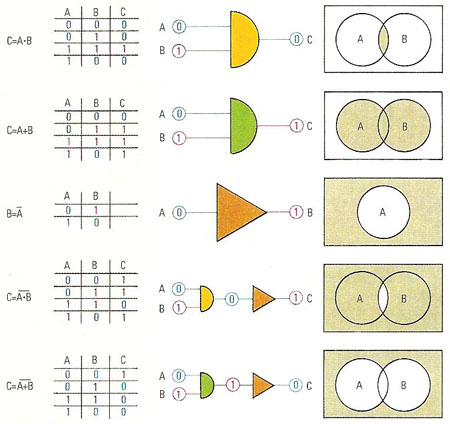
\includegraphics[width=.75\textwidth]{Boolean_algebra}}
	\end{figure}
\end{frame}



\begin{frame}{Boolean Data Type}
\begin{block}{Declaration}
	\begin{center}
		\item \textcolor{DarkOrchid}{\textbf{bool}} \textit{A};\\
		\item \textcolor{DarkOrchid}{\textbf{bool}} \textit{B};
		\item \textcolor{DarkOrchid}{\textbf{bool}} \textit{C};
	\end{center}
\end{block}
\pause
\begin{block}{Assignment}
	\begin{align*}
		A &= \textcolor{RoyalBlue}{\textbf{true}};\\
		B &= \textcolor{RoyalBlue}{\textbf{false}};
	\end{align*}
\end{block}
\end{frame}

\begin{frame}{Boolean Algebra: Not}
	\begin{figure}
		\href{http://www.daviddarling.info/encyclopedia/B/Boolean_algebra.html}{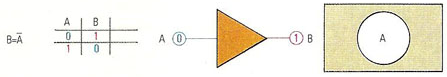
\includegraphics[width=1\textwidth]{not}}
	\end{figure}
	\pause
	\begin{block}{C++}
		\begin{center}
			{\LARGE B = \textcolor{red}{!}A;}
		\end{center}
	\end{block}
\end{frame}

\begin{frame}{Boolean Algebra: And}
	\begin{figure}
		\href{http://www.daviddarling.info/encyclopedia/B/Boolean_algebra.html}{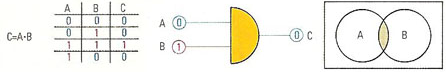
\includegraphics[width=1\textwidth]{and}}
	\end{figure}
	\pause
	\begin{block}{C++}
		\begin{center}
			{\LARGE C = A\textcolor{red}{\&\&}B}
		\end{center}
	\end{block}
\end{frame}

\begin{frame}{Boolean Algebra: Not And}
\begin{figure}
		\href{http://www.daviddarling.info/encyclopedia/B/Boolean_algebra.html}{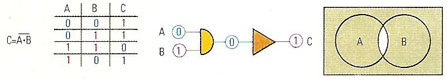
\includegraphics[width=1\textwidth]{not_and}}
	\end{figure}
	\pause
	\begin{block}{C++}
		\begin{center}
			{\LARGE C = \textcolor{red}{!}(A\textcolor{red}{\&\&}B) }
		\end{center}
	\end{block}

\end{frame}

\begin{frame}{Boolean Algebra: Or}
\begin{figure}
		\href{http://www.daviddarling.info/encyclopedia/B/Boolean_algebra.html}{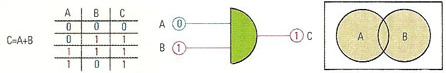
\includegraphics[width=1\textwidth]{or}}
\end{figure}
\pause
	\begin{block}{C++}
		\begin{center}
			{\LARGE C = A\textcolor{red}{$\mid\mid$}B}
		\end{center}
	\end{block}
\end{frame}

\begin{frame}{Boolean Algebra: Not Or}
\begin{figure}
		\href{http://www.daviddarling.info/encyclopedia/B/Boolean_algebra.html}{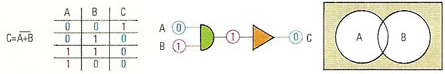
\includegraphics[width=1\textwidth]{not_or}}
	\end{figure}
	\pause
	\begin{block}{C++}
		\begin{center}
			{\LARGE C = \textcolor{red}{!}(A\textcolor{red}{$\mid\mid$}B)}
		\end{center}
	\end{block}
\end{frame}

\begin{frame}{De Morgan's Law}
	\begin{align*}
	\textcolor{red}{!}(A\textcolor{red}{\&\&}B)  &= (\textcolor{red}{!}A \textcolor{red}{\mid\mid}\textcolor{red}{!}B)\\
	\textcolor{red}{!}(A\textcolor{red}{\mid\mid}B)  &= (\textcolor{red}{!}A \textcolor{red}{\&\&}\textcolor{red}{!}B)
	\end{align*}
\end{frame}

\begin{frame}{Relational Operator}
	\begin{figure}
		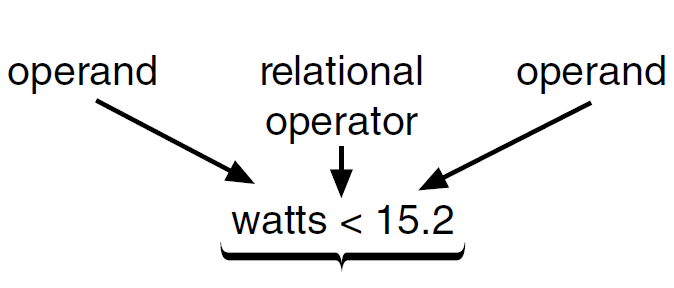
\includegraphics[width=.5\textwidth]{ops}
	\end{figure}
	\pause
	\begin{center}
	\begin{tabular}{|c|l|}
		\hline
		\textbf{Operator} & \textbf{Meaning}\\
		\hline
		\textless & less than \\
		\textless= & less than or equal \\
		\textgreater & greater than \\
		\textgreater= & greater than or equal \\
		== & equal  \\
		!= & not equal \\
		\hline
	\end{tabular}
	\end{center}
\end{frame}

\begin{frame}{Comparing Characters}
	\begin{itemize}
		\item comparison is done between ASCII encodings 
		\item words are compared on a character basis
		\item C++ provides functions for comparing characters
	\end{itemize}
\end{frame}

\begin{frame}{Comparing Doubles and Floats}
	\begin{block}{Roundoff Errors}
		\begin{description}
			\item[FALSE] 1/3.0 == 0.333333333333333
			\item[TRUE] 1/3.0 == 0.3333333333333333
		\end{description}
	\end{block}
	\pause
	\begin{block}{Avoiding Roundoff Errors}
		\begin{itemize}
			\item abs(1/3.0 – 0.333333333333333) < epsilon
			\item epsilon is a constant set to a teeny tiny value
		\end{itemize}
	\end{block}
\end{frame}

\begin{frame}{Practice}
Write relational expressions to express the following conditions (using variable names of your choosing):
	\begin{itemize}
		\item The distance is equal to 30 feet.	
		\item The ambient temperature is 86.4 degrees.
		\item A speed is 55 mph.
		\item The current month is 12 (December).
		\item The letter input is K.
		\item A length is greater than 2 feet and less than 3 feet.
		\item The current day is the 15th day of the 1st month.
		\item The automobile’s speed is 35 mph and its acceleration is greater than 4 mph per second.
		\item An automobile’s speed is greater than 50 mph and it has been moving for at least 5 hours.
		\item The code is less than 500 characters and takes more than 2 microseconds to transmit.
	\end{itemize}
\end{frame}

\end{document}

